\chapter{Systembeskrivelse}
Dette afsnit beskriver det implementerede system. \\
\noindent Systemet BargainBarter er en webapplikation der hostes på \url{http://10.29.0.30/BargainBarter} på AU's netværk. Denne hjemmeside tilbyder brugere at oprette en brugerprofil, hvorefter de får mulighed for at benytte kernen af hjemmesidens funktionaliteter. \\ \\ \noindent
En af kernefunktionaliteterne er at kunne oprette en annonce, med det formål at kunne bytte artiklen i annoncen med andre artikler. Annoncen består af et billede af artiklen, en titel, en beskrivelse samt hvilken kategori den hører under. Når denne annonce er oprettet bliver den tilgængelig på det samlede overblik af annoncer på forsiden. Ved at klikke på en annonce har brugeren mulighed for at få nærmere detaljer omkring den pågældende artikel. Herfra har en bruger adgang til informationer om sted/adresse på den pågældende brugers annonce, afstand til brugeren, offentlige kommentarer på annoncen, brugerens byttehistorik og vurderinger fra andre brugere på baggrund af tidligere byttehandler. \\ \\ \noindent
Via et fælles chatrum har brugerne af hjemmesiden mulighed for at kunne kommunikere med hinanden på kryds og tværs og evt. aftale tid og sted for en byttehandel. \\ \\ \noindent
Figur \ref{fig:rigbillede} viser et scenarie på en byttehandel mellem to brugere.

\begin{figure}[H]
	\centering
	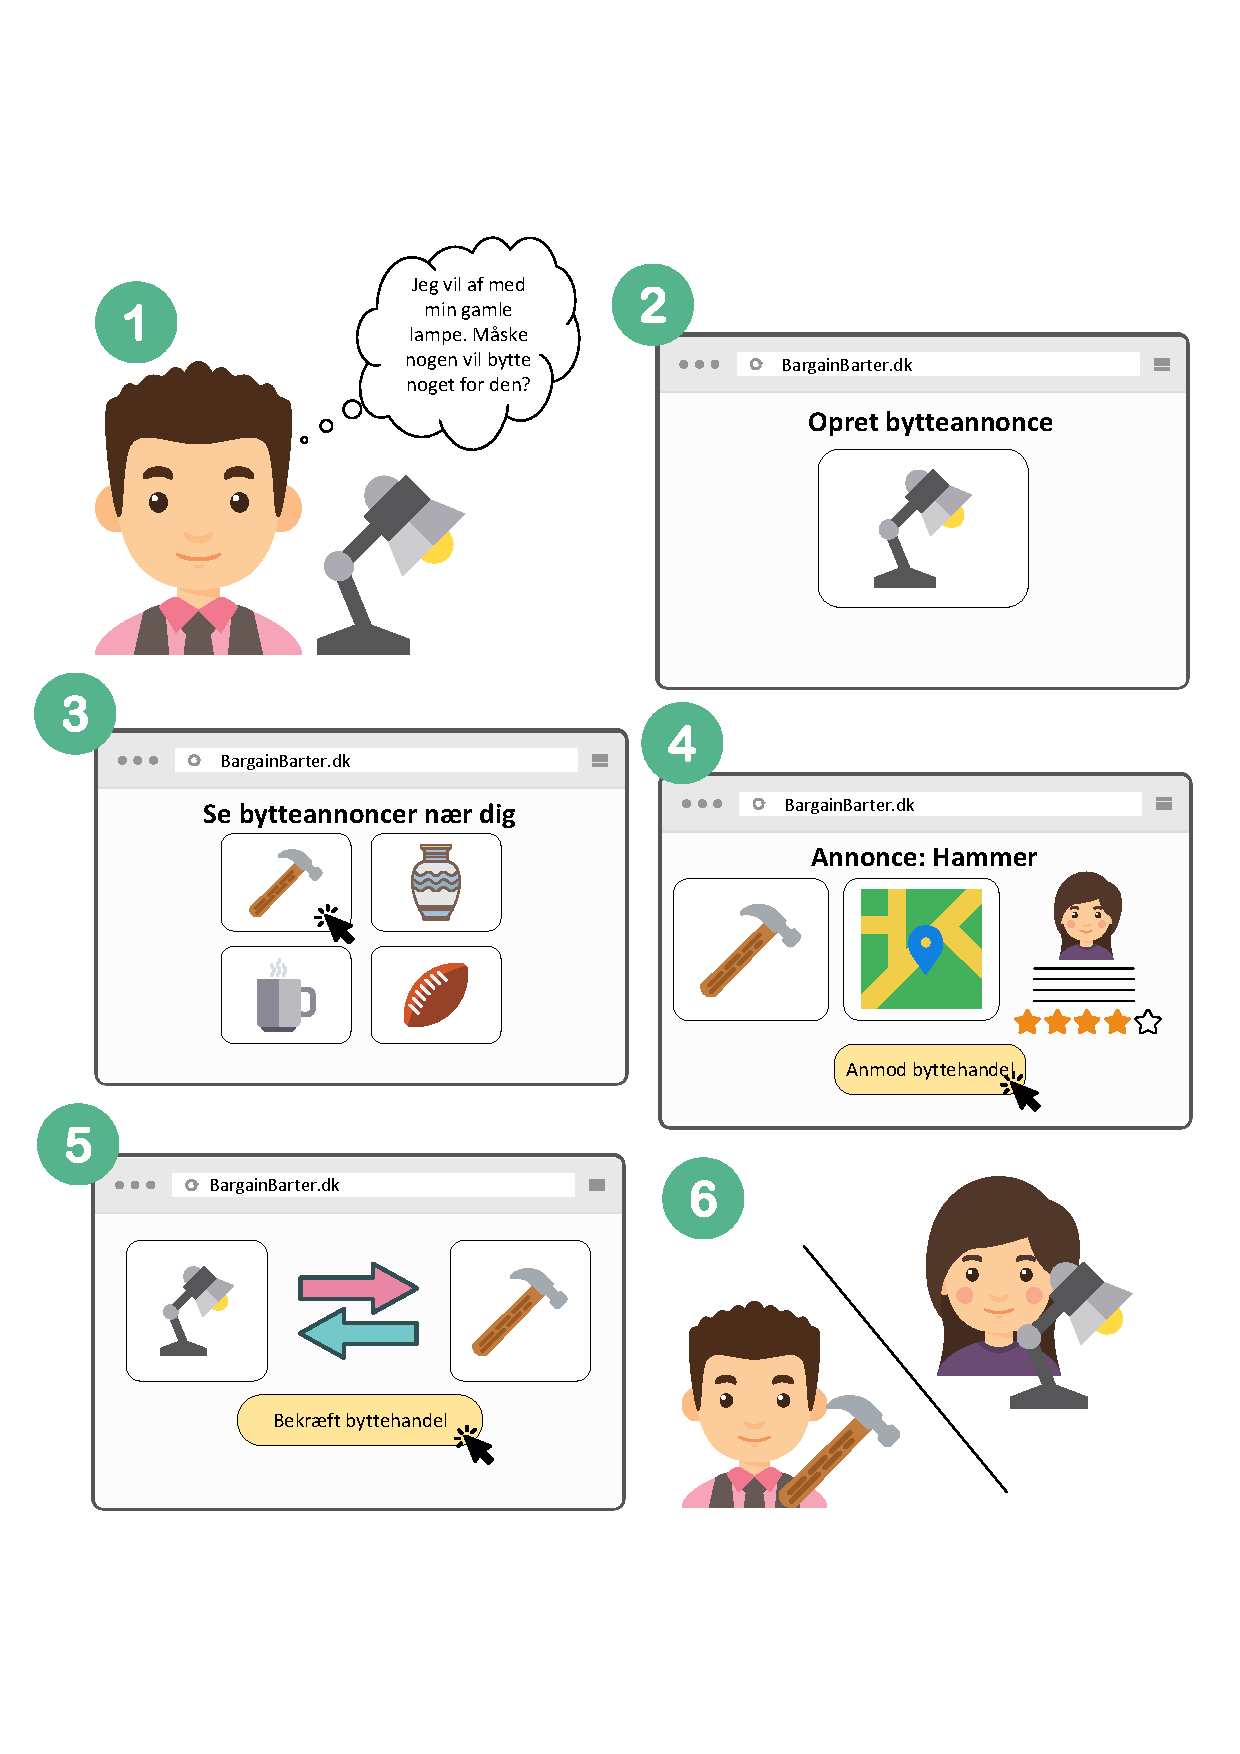
\includegraphics
	[width=140mm]{figures/rigtbillede_version1.pdf}
	\caption{Scenarie for byttehandel}
	\label{fig:rigbillede}
\end{figure} 
